\documentclass[a4paper]{article}

\usepackage[utf8]{inputenc}
\usepackage{erk}
\usepackage{times}
\usepackage{graphicx}
\usepackage[top=22.5mm, bottom=22.5mm, left=22.5mm, right=22.5mm]{geometry}

\usepackage[slovene,english]{babel}
\usepackage{hyperref}
\usepackage{url}

\let\oldfootnotesize\footnotesize
\renewcommand*{\footnotesize}{\oldfootnotesize\scriptsize}

\begin{document}
\title{MoveZeBall}

\author{Domen Lanišnik, Anže Kovač} % use ^1, ^2 for author(s) from different institutions

\affiliation{Univerza v Ljubljani, Fakulteta za računalništvo in informatiko \\}

\email{E-pošta: dl8359@student.uni-lj.si, ak9427@student.uni-lj.si}

\maketitle

\selectlanguage{slovene}

\begin{abstract}{Abstract}
Igra premikanja žoge skozi poligon ali MoveZeBall, je 3D igra narejena na osnovi WebGL in s pomočjo JavaScript knjižnjic Three.js \footnote{\url{https://github.com/mrdoob/three.js/}} in Cannon.js \footnote{\url{https://github.com/schteppe/cannon.js/}}. Igra od uporabnika zahteva uporabo fizičnih lastnosti sveta ter njegovo spretnost in zmožnost prilagajanja na nenadne spremembe. Cilj igre je žogo pripeljati uspešno do cilja.
\end{abstract}


\section{Pregled igre}
\begin{figure}[!htb]
    \begin{center}
        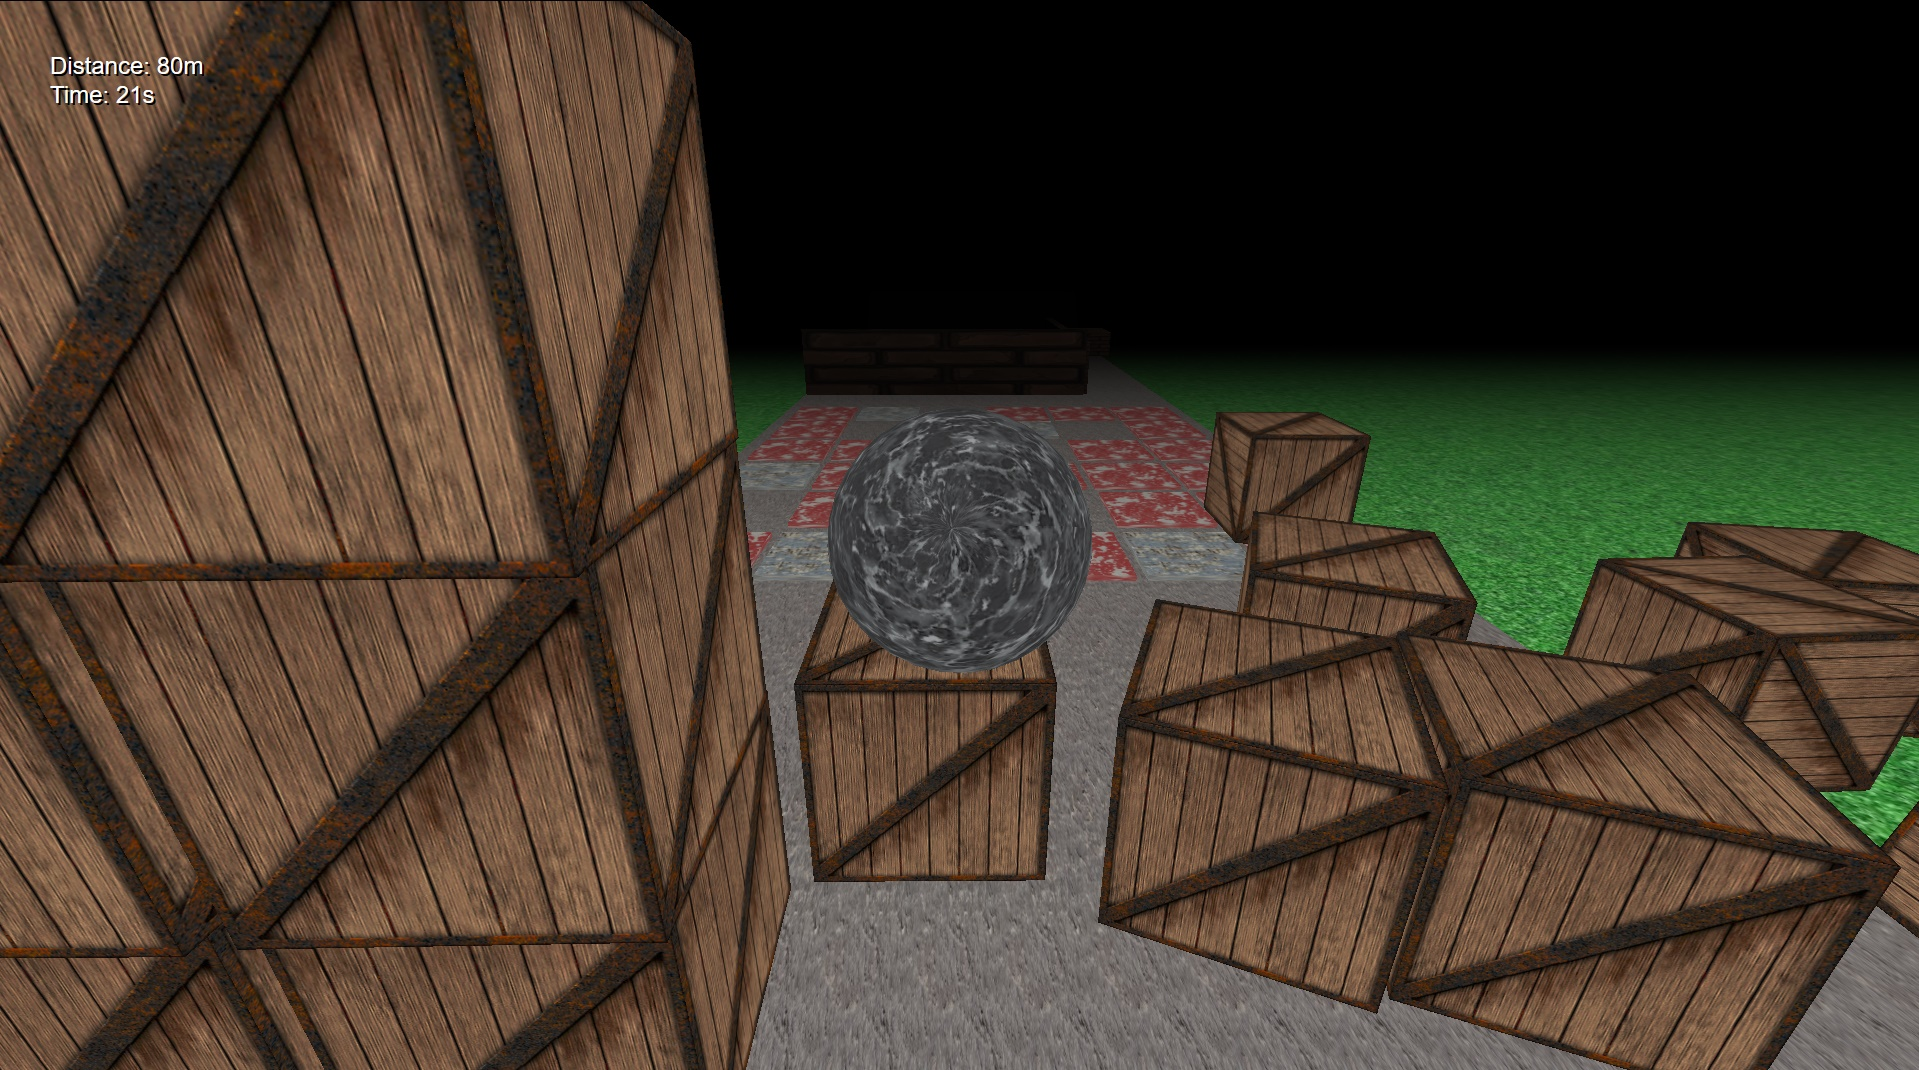
\includegraphics[width=\columnwidth]{moveZeBall.jpg}
        \caption{Opravljena prva ovira.} \label{fig:slika}
    \end{center}
\end{figure}
Igra MoveZeBall\ref{fig:slika} je avanturni žanr igre, v kateri igramo v vlogi marmorne krogle, ki se je znašla v svetu s štirimi preprekami, ki jih moramo premagati, da se prebijemo do končne ciljne platforme, kjer se lahko vpišemo med najboljše igralce. 

Poleg težkih ovir, ki jim moramo biti kos, pa nas vseskozi spremlja tudi nevarnost dotika trave oziroma premičnih stenskih kock, ki pomenita takojšen konec igre. 

Igra je za nove igralce zelo zahtevna in od igralca zahteva veliko potrpežljivosti in ne prenagljenih dejanj. V nasprotnem primeru se lahko hitro spet znajde na začetku. Igra je namenjena vsem, ki si želijo preizkusiti kako jekleni so njihovi živci, in tudi tistim, ki iščejo le zabavo. 

Igra se odvija na ravnini, ki je obdana z gorami, ki jih lahko ves čas vidimo v ozadju. Celotna zgodba temelji na žogi, ki jo je potrebno pripeljati do cilja, brez da vmes pademo na nevarno travo ali se dotaknemo odbijajočega zidu. Če nam uspe premagati tudi nepredvidljive plošče in ohraniti ravnotežje na mostu iz škatelj, smo na koncu nagrajeni z lepim razgledom in vpisom na lestvico najboljših.  Scenarij za igro je ta, da z žogo premagujemo zadane ovire v čim hitrejšem možnem času.


\subsection{Opis sveta}
Celoten svet se odvija v horizontalni liniji, kar pomeni, da se igra odvija s tem ko napredujemo s premikanjem naprej, kjer vseskozi srečujemo nove ovire. Pri celostnem stilu igre, sva poizkušala čimbolj ponazoriti realističen svet s pomočjo tekstur. Prav tako svet obdaja skybox, ki daje občutek boljše umeščenosti v prostor. Žoga, ki je glavni lik te igre se lahko premika v katerikoli smeri v 3D prostoru, kar pomeni, da imamo na voljo premikanje v vse smeri, kot tudi možnost skakanja.

\subsubsection{Pregled}
Svet, s katerim ima igralec stik je kamnita površina. Te ne smemo zapustiti, saj je obdana s travo, katere dotik pomeni konec igre. Zaporedno si na tej površini sledijo ovire, katere je potrebno včasih tudi kombinirati med seboj, da uspemo premagati naslednjo oviro. Vsaka ovira, ki sledi je zahtevnejša od prejšnje.

\subsubsection{Ozadje}
\begin{figure}[!htb]
    \begin{center}
        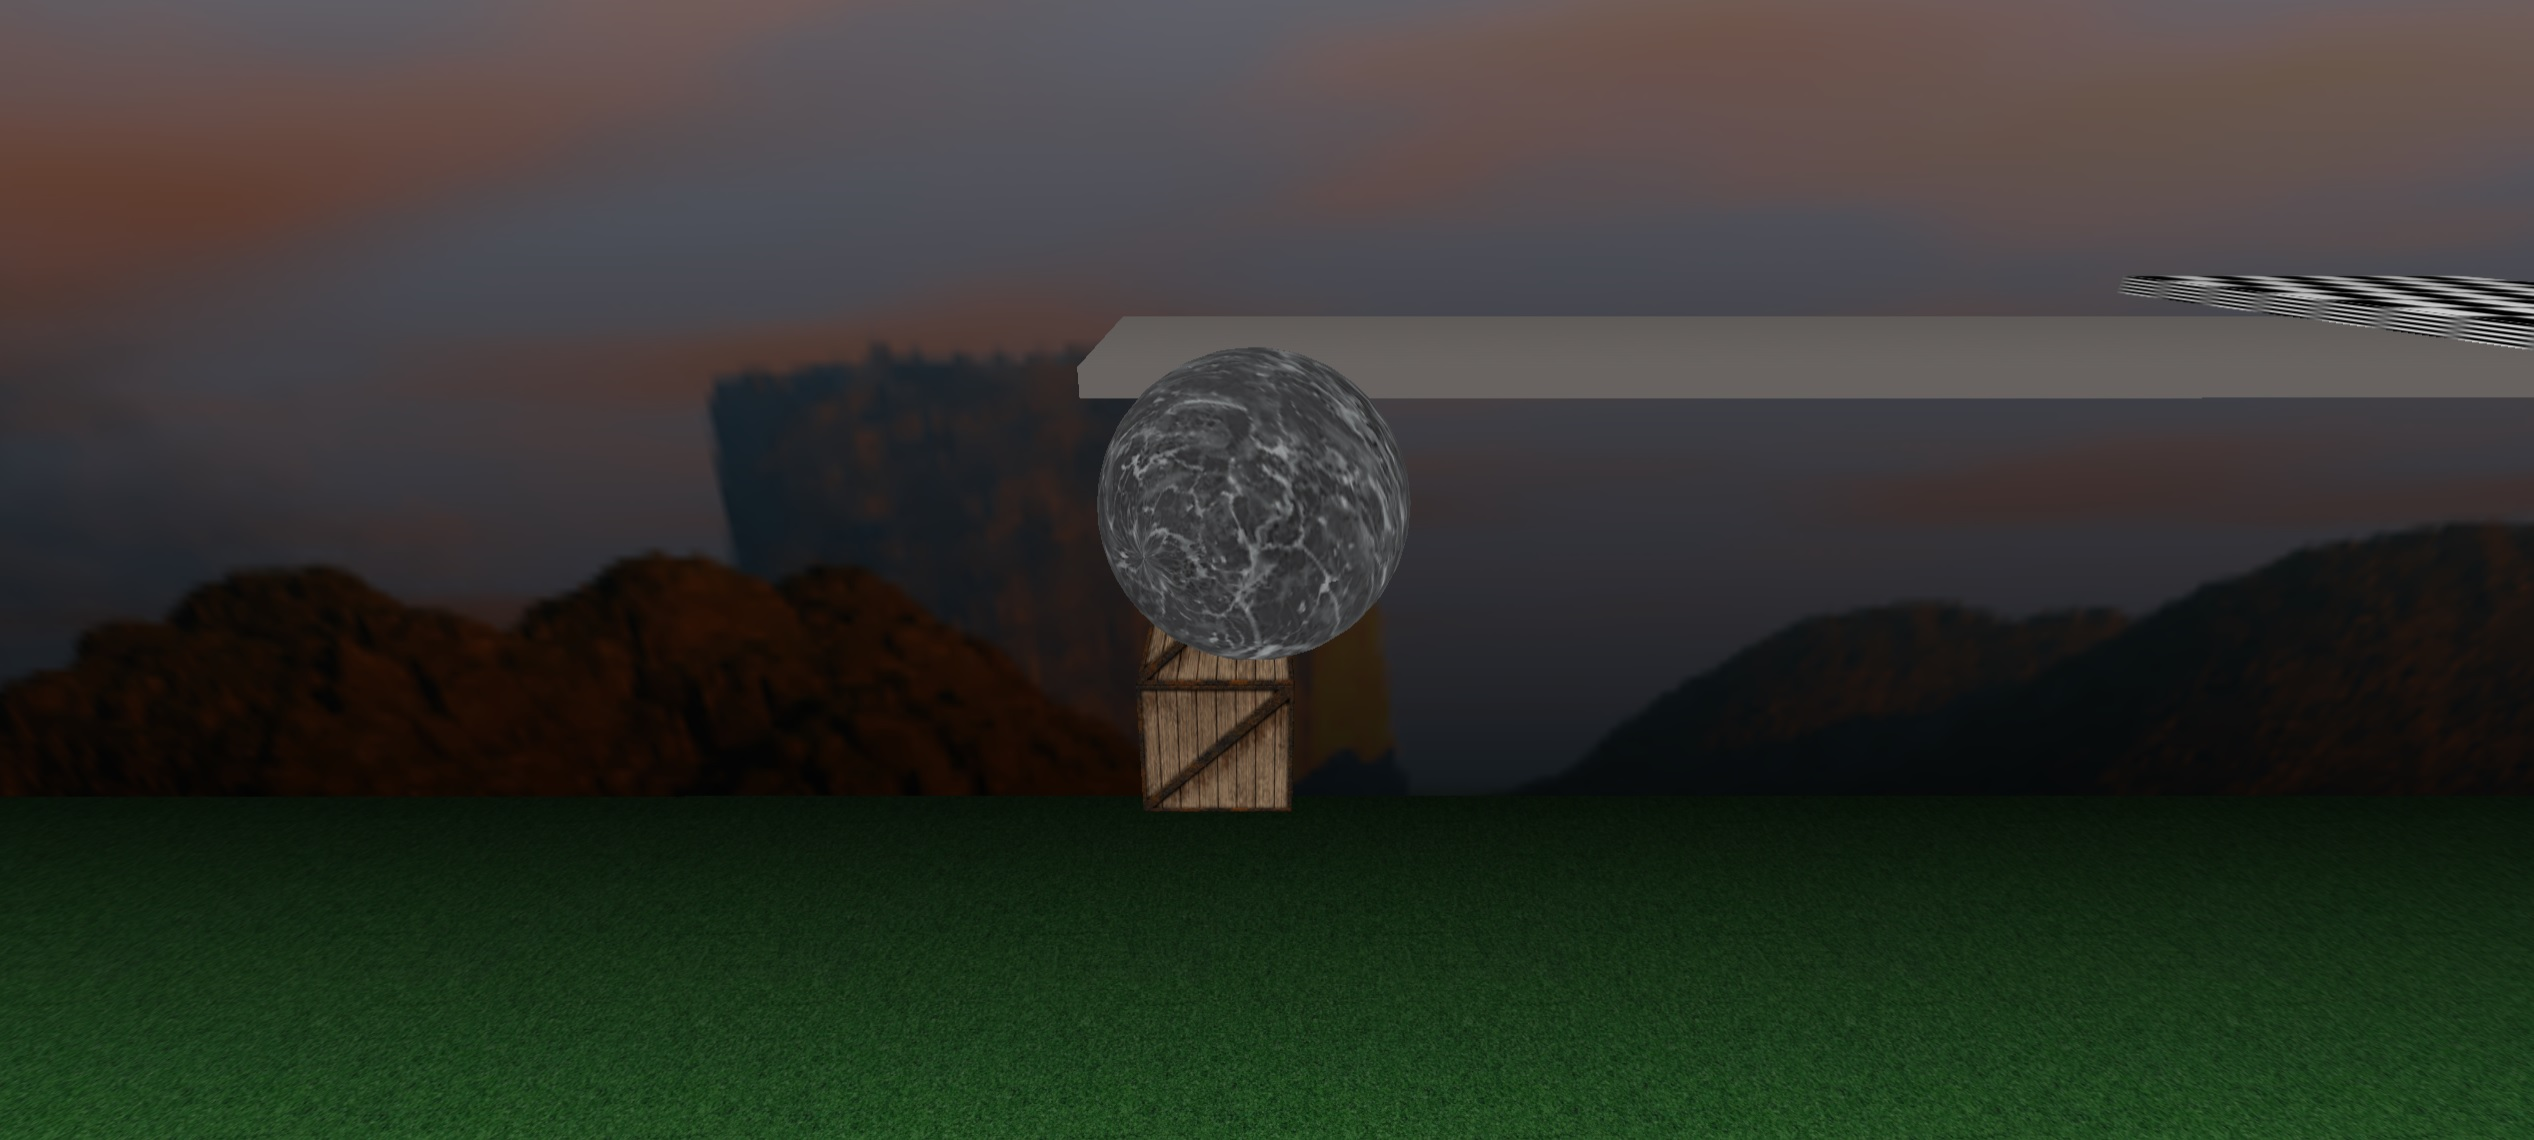
\includegraphics[width=\columnwidth]{finish.jpg}
        \caption{Pogled na ciljno ravnino.} \label{fig:konec}
    \end{center}
\end{figure}
Ozadje v igri predstavljata travnata ravnina, ki se razprostira na obe smeri od igralne linije, kot tudi nebo in ozadje, ki spominja na gore oziroma gorsko področje. Vseskozi čez igro to okolico vidimo zelo slabo. Ker se ji ne moremo približati tako, da gremo čez travo, je naša edina opcija napredovanje naprej, kjer se vse bolj približujemo tej okolici, in ko smo na končni platformi lahko vidimo okolico v vsej svoji lepoti. To je tudi ena izmed nagrad za uspešno opravljeno igro. S tem sva želela okolico vključiti neposredno v igro in zgodbo četudi se gre za statični objekt.

\subsubsection{Ključne lokacije}
Ključne lokacije v igri so osnovna igralna ploskev na katero so postavljene ovire, potem pa so ključne lokacije posamezne ovire, ki jih moramo premagati. Ovire so nihajoča veriga, ki jo mora uporabnik izkoristiti da lahko podre drugo oviro, ki je zid iz zabojev, katerega ne more preskočiti zaradi višine. Naslednja ključna lokacija so nepredvidljive plošče, ki služijo kot minsko polje. Ob stiku z rdečo ploščo, žogo odstreli nazaj do zidu, kjer moramo znova poizkusiti. Ob stiku s sivo ploščo, pa se nam zamenjajo kontrolne tipke, kar v zelo ozkem in natančnem prostoru lahko predstavlja problem, če se ne prilagodimo zelo hitro. 

Naslednja ovira je zid, iz katerega se kocke v definiranem vrstnem redu premikajo naprej in nazaj. Pot lahko vodi le mimo teh premikajočih kock. Ob stiku s katero od kock smo zaključili z igro. 

Naslednja ovira je vzpetina, na katero se moramo vzpeti. Za vzpetino pa se nam razprostre pogled na statične lebdeče dele mostu preko katerih moramo skakati in paziti da ne pademo v globino na travo. 

Zadnja ključna lokacija pa je še ciljna ravnina in končna platforma, kjer se uspešno zaključi naša igra.

\subsubsection{Velikost}
Ker sva s samim stilom igre želela prikazati čim bolj realno podobo, je tudi velikost sveta definirana kot zunanja pokrajina gledana z vidika človeka. V igri so definirani zaboji, zid in plošče, ki poizkušajo ponazoriti vsakodnevno človeško okolico. Tudi okolica se sklada z opisano velikostjo, saj igramo v nekakšni dolini obdani z gorovjem. Sama merska enota s katero merimo uspešnost igralca so metri, kar pomeni, da lahko rečemo, da gre za žogo v velikosti človeka.

\subsubsection{Objekti}
V igri so uporabljeni objekti, ki združeni skupaj predstavljajo naprednejše strukture. Osnovni objekt je kotaleča krogla z implementiranim mehkim zavijanjem in možnostjo navigiranja v več smeri hkrati (npr. naprej in levo).

Krogla ima teksturo marmorja, s čimer igralec dobi občutek prestižnosti krogle in hkrati strah, da se krogla ne razbije če pade s prevelike višine.  

Objekti v nihajoči verigi so lesene plošče, ki so skupaj zvezane s tečaji, ki se lahko premikajo. 
Objekti v zidu so leseni zaboji, ki imajo vključeno dinamičnost, kar pomeni da jih lahko premikako oziroma podremo strukturo v katero so zgrajeni. 

Naslednji objekt so plošče, ki so kvadratne oblike in s svojo barvo opozarjajo na nevarnost. Bolj nevarne so rdeče plošče, ki katapultirajo v zrak in nazaj, medtem ko so manj nevarne plošče sive, ki nam le zamenjajo kontrole. 

Zaporedje otočkov po katerim moramo skakati da pridemo do zadnje platforme so prav tako v zraku statično pritrjene podolgovate lesene škatlje, katere so narejene tako, da lahko igralec zavira hitrost žoge pred naslednjim skokom.

 Zadnji  in ciljni objekt pa je platforma ovita v teksturo kariraste zastave, ki predstavlja konec.

\subsubsection{Čas}
Čas v igri teče tako kot v realnosti. 1 sekunda v realnem svetu je 1 sekunda v igri. Eden od ključnih parametrov pri uspešnosti v igri je tudi koliko časa smo porabili, da smo prišli do konca. Ker kot končni rezultat se nam ne vpiše, kako daleč po prišli, ampak se nam izračuna uspešnosti koeficient, ki upošteva tudi čas, ki smo ga porabili da smo prišli tako daleč.

\subsection{Igralni pogon in uporabljene tehnologije}
Uporabljen igralni pogon je WebGL. Za lažji razvoj pa sva uporabili JavaScript knjižnico Three.js , ki ponuja ogrodje za lažje in hitrejše kreiranje in urejanje objektov. Poleg osnovne knjižnice sva uporabila tudi fizikalni pogon Cannon.js, ki omogoča, da elementom dodamo dinamičnost, gravitacijo in vse ostale fizične lastnosti, ki naredijo objekt takšen, da imamo občutek kot da se nahajo v realnem svetu. 
Poleg teh dveh tehnologij je uporabljena tudi funkcionalnost WebStorage, ki ga ponuja JavaScript za shranjevanje najboljših dosežkov.

\subsection{Pogled}
Pogled v igri je statično nameščen glede na pozicijo žoge. Kamera se vedno nahaja za in nad žogo s pogledom usmerjenim proti žogi. Ob zavijanju se kamera rahlo zarotira v smer v katero zavijamo. Kamera sledi žogi ob vseh akcijah.

\section{Osebek}
Glavni osebek v igri je marmorna žoga, ki jo upravljamo skozi ovire. Ob enem je to tudi edini osebek nad katerim imamo v igri nadzor. Upravljanje osebka je povsem preprosto in ituitivno. Premikanje v vseh smereh izvajamo s pomočjo smernih tipk, za skakanje pa je namenjena preslednica oziroma  `Space`.  Dvojni skoki so onemogoči, s čemer onemogočimo preskakovanje visokih ovir. Krogla se dinamično odziva na okolico. Z njo lahko podremo zid. Ob kontaktu plošč jo katapultira na začetek. Zbije jo lahko kocka, ki skoči iz zidu. Glavna akcija, ki pa je tudi cilj igre, je ta, da se dotakne končne ciljne plošče, s čimer se zaključi igra.


\section{Uporabniški vmesnik}
Uporabniški vmesnik je preprost in nevsiljiv. Na začetku igre se nam prikažejo navodila kako igrati z izpisanimi kontrolami. Ta vmesnik vsebuje tudi gumb za pričetek igre. Vseskozi med igranjem imamo v zgornjem levem kotu prikazano kako daleč od izhodišča smo prišli. Prav tako se nam prikazuje porabljen čas. V primeru konca igre oziroma da osvojimo ciljno platformo, se nam prikaže obvestilo o koncu igre in našem rezultatu. Ponujene so možnosti ponovne igre ali vpisa med najbolše igralce. Za tem se celotna stvar ponovi od začetka.

\section{Glasba in zvok}
Glasbe v igri nisva uporabila, kajti igra zahteva veliko koncetracije. Veliko ljudi pa moti igranje glasbe, zato le te nisva vključila.

\section{Gameplay}
Igra se prične na začetku steze, ki je obdana s trav,o pred nami pa vidimo že prvi dve oviri. Za sam začetek moramo v meniju izbrati opcijo za začetek igre. Ko se igra prične, moramo s kombinacijo smernih tipk in skokov upravljati žogo tako, da pridemo čim dlje po poligonu. Ob tem moramo paziti na nepredvidljive plošče, ki nas katapultirajo na začetek oziroma na premikajoče kocke iz stene, ob stiku s kateremi se igra takoj konča. Pri preskakovanju iz otočka na otoček pri zadnji oviri pa je vse kar moramo narediti to, da ohranimo mirne živce. Vseskozi se nam računati tudi količnik uspešnosti, ki je razmerje med razdaljo od začetka, ki smo jo že opravili in časom, ki smo ga za to potrebovali. Igra se uspešno konča ob dotiku zadnje ciljne plošče, kjer se nam prikaže lep razgled in možnost vpisa med najboljše igralce. Možnost vpisa med najboljše igralce se nam pojavi tudi, če igro predčasno zaključimo, toda naš količnik uspešnosti zagotovo ne bo visok in se ne bomo uvrstili med najboljše igralce.


\section{Zaključki in možne nadgradnje}
Pri izdelavi igre sva se naučila samostojnega razvoja spletne WebGL igre. Naučila sva se, kako načrtovati idejo, ki jo je možno realizirati z znanjem, ki ga imava na voljo in kako implementirati 3D fiziko v igro. Naučila sva se, kako izračunati, da premikanje objekta ne sledi le ravnim črtam ampak da je pot podobna loku. Prav tako sva se naučila pridobivanja in urejanja tekstur in njihove uporabe, za shranjevanje rezultatov pa sva se naučila tudi uporabe WebStorage funkcionalnosti. Veliko primerov sva našla tudi v knjigi \cite{dirksen2013learning}

Igro bi bilo zagotovo mogoče nadgraditi z boljšimi in bolj prilegajočimi teksturami, dodanih bi bilo lahko več izzivov, med katerimi bi bil lahko kakšen, ki je dinamično generiran. Prav tako bi lahko okolico zapolnjevalo več dodatnih statičnih elementov.

Končna igra se od začetne ideje ne razlikuje veliko. Zaradi pomanjkanja časa sva spustila možnost več življenj in porabljanja energije pri premikanju.


\small
\bibliographystyle{plain}
\bibliography{references}

\end{document}
